\documentclass[12pt, draft]{beamer}
\usetheme{Darmstadt}

\usepackage[utf8]{inputenc}
\usepackage[german]{babel}
\usepackage[T1]{fontenc}
\usepackage{amsmath}
\usepackage{amsfonts}
\usepackage{amssymb}
\usepackage{tikz}
\usepackage{tabularx}

\title{Implementation eines Blokus-Spielers}
\author{\mbox{Lukas Jagemann}}
\date{\today}


\begin{document}

\begin{frame}
    %\begin{figure}[h]
    %    \centering
    %    \resizebox{0.5\linewidth}{!}{\includegraphics{../media/logo.eps}}
    %\end{figure}
    \vspace*{-20pt}
    \titlepage
\end{frame}

\begin{frame}{Inhalt}
	\setcounter{tocdepth}{1}
    \tableofcontents
\end{frame}

\section{Blokus}
\subsection{Überblick}
\begin{frame}
	Entstanden $\sim$2000\\
	Ursprünglich für 4 Spieler
    \begin{figure}[tp]
        \centering
        \resizebox{0.7\linewidth}{!}{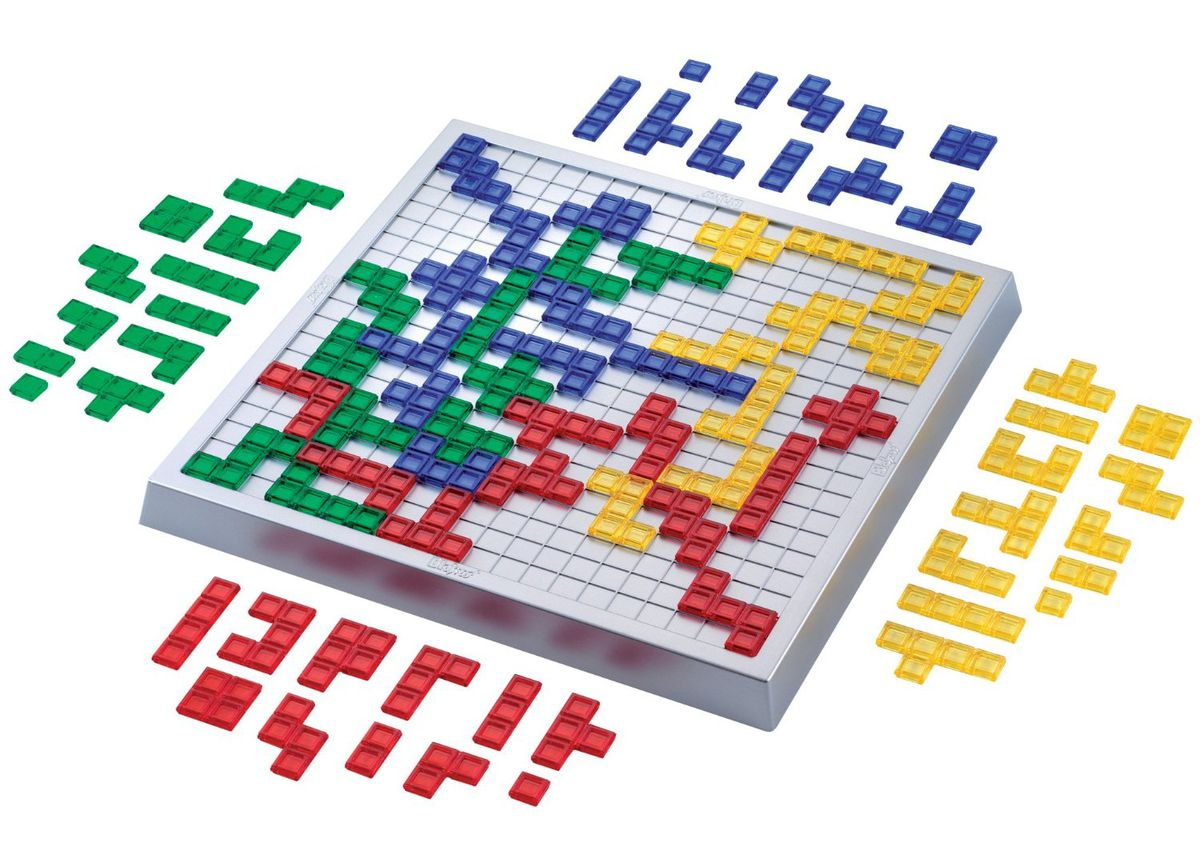
\includegraphics[width=\linewidth]{media/blokus4p.jpg}}\\
        \tiny Quelle: \url{https://media.takealot.com/covers\_tsins/32082437/81LEjjVViUL.\_SL1500\_-zoom.jpg}
    \end{figure}
\end{frame}
\begin{frame}
	\begin{tabularx}{\hsize}{*2{>{\centering\arraybackslash}X}}
		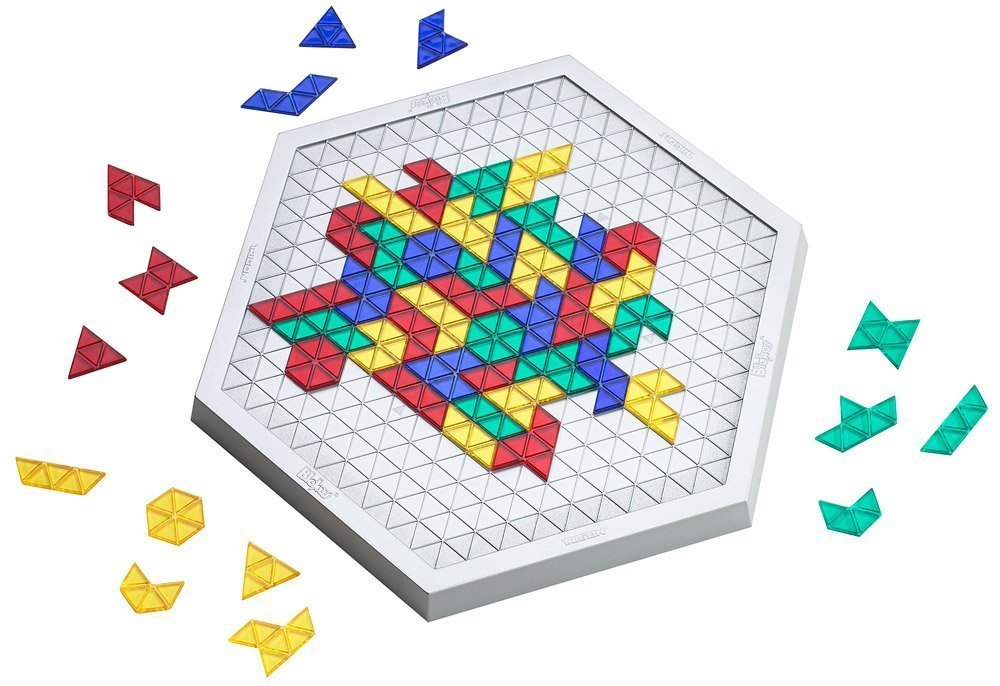
\includegraphics[width=\linewidth]{media/blokus3p.jpg}\linebreak
		\tiny Quelle: \url{http://www.passionforpuzzles.com/weblog/wp-content/uploads/2010/12/613KSlRx9oS._SL1500_.jpg}
	    &
		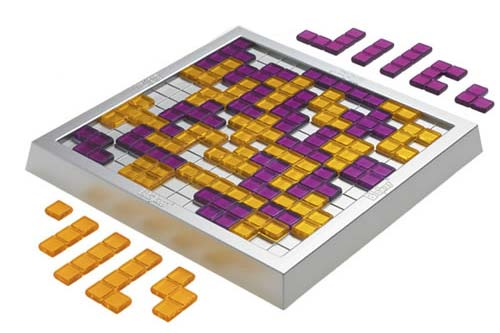
\includegraphics[width=\linewidth]{media/blokus2p.jpg}\linebreak
		\tiny Quelle: \url{http://boardgaming.com/wp-content/uploads/2012/02/blokus-duo-game-in-play.jpg}
	\end{tabularx}
\end{frame}
% Entstanden ~2000 als 4 spieler gemeinschaftsspiel
% 
\subsection{Wie man spielt} \begin{frame}\end{frame}
\subsection{Wie man startet} \begin{frame}\end{frame}
\subsection{Online Ressourcen} \begin{frame}\end{frame} % ?

\section{Das Projekt}
\subsection{Wunderschönes CSS3 und HTML5} \begin{frame}\end{frame}
% valide
\subsection{TypeScript, das bessere JavaScript} \begin{frame}\end{frame}
% classen
% strenges typsystem
% ide support
% einheitlicher kompiler -> es3,5,6,...
\subsection{Code Struktur} \begin{frame}\end{frame}
\subsection{GameState} \begin{frame}\end{frame}
% History slider
% Saving states

\section{Minimax}
\subsection{Wie funktioniert MiniMax} \begin{frame}\end{frame}
% Ziel: beide spieler spielen optimal
\subsection{Grafische Veranschaulichung} \begin{frame}\end{frame}
\subsection{Wann MiniMax gut funktioniert} \begin{frame}\end{frame}
% Geringes branching
% Berechenbarer status
% (oft gegen ende stark)
\subsection{...und wann eher weniger} \begin{frame}\end{frame}
% hohes branching
% wenig 
\subsection{Abwandlungen} \begin{frame}\end{frame}
% aplha beta heuristiken

\section{Die Logik}
\subsection{Konzept} \begin{frame}\end{frame}
\subsection{Gewichtung: Bits} \begin{frame}\end{frame}
\subsection{Gewichtung: Ecken} \begin{frame}\end{frame}
\subsection{Gewichtung: TrueLength} \begin{frame}\end{frame}
\subsection{Gewichtung: Weitestes Feld} \begin{frame}\end{frame}
\subsection{Gewichtung: Erreichbare Felder} \begin{frame}\end{frame}
\subsection{Gewichtung finden} \begin{frame}\end{frame}
% Selber nachdenken
% Erfahrung
% Problem: Unnormierte Werte
\subsection{...oder finden lassen} \begin{frame}\end{frame}
% Genetic failure :P

\section{Optimierungen}
% Javascript...
\subsection{Problem: MiniMax Tiefe?} \begin{frame}\end{frame}
% hohe kosten für evaluation
\subsection{Lösung: Adaptiver MiniMax} \begin{frame}\end{frame}
% zacken diagramm
\subsection{Berechnungen wiederverwenden} \begin{frame}\end{frame}
\subsection{und notfalls löschen} \begin{frame}\end{frame}
\subsection{Multithreading (oder so)} \begin{frame}\end{frame}
\subsection{Inkrementelle GameStates} \begin{frame}\end{frame}

% + alpha/beta

\section{Mögliche Optimierungen (Ausblick)}
\subsection{Kleine Steine am Anfang ignorieren} \begin{frame}\end{frame}
\subsection{Dynamische Gewichtung} \begin{frame}\end{frame}
\subsection{Summen-Erreichbare Felder} \begin{frame}\end{frame}
% bla
% =======
\subsection{Anderer Algorithmus?} \begin{frame}\end{frame}
% Bild mit den zwei einsern
% Monte carlo ?
% sehr stark heuristik basierend
\subsection{Priorisieren von Gebieten in MiniMax} \begin{frame}\end{frame}
% Mehr Rechenleistung in interessante Gebiete stecken
\subsection{Neuschreiben, in einer besseren Sprache} \begin{frame}\end{frame}
% Performance, Memorymanagemenet, Threads

\end{document}